
\section{Software solutions and languages for AP and DSS - 29.09.22}


% Decisioni operative/strutturate
\subsection{Decisioni operative/strutturate}

Sono una classe importante, \hl{si possono prendere tramite una procedura standard} che può seguire un manuale o delle normative, automatizzata o no. Queste decisioni di breve periodo si collocano in basso a destra in figura  \ref{diadec}.

Non essendo decisioni dove possiamo solo supportare, allora si possono andare a \hl{codificare in un linguaggio di programmazione procedurale} come C++, Java, ecc...

Potremo avere un \hl{approccio}:

\begin{itemize}
	\item \hl{procedurale}: dove devo far \textbf{generare delle azioni} in seguito di un obiettivo
	
	\item \hl{dichiarativo}: si divide in:
		\begin{enumerate}
			\item \textbf{modellazione} del problema
			
			\item \textbf{descrivo tramite un linguaggio di modellazione} (modelling language) che è un linguaggio di programmazione matematico come AMPL, oppure in linguaggi come python con Amply e Pulp
			
			\item \textbf{solver of the shelf}, che ci darà delle istruzioni per il nostro contesto
		\end{enumerate}
\end{itemize}


\begin{figure}[H]
\centering
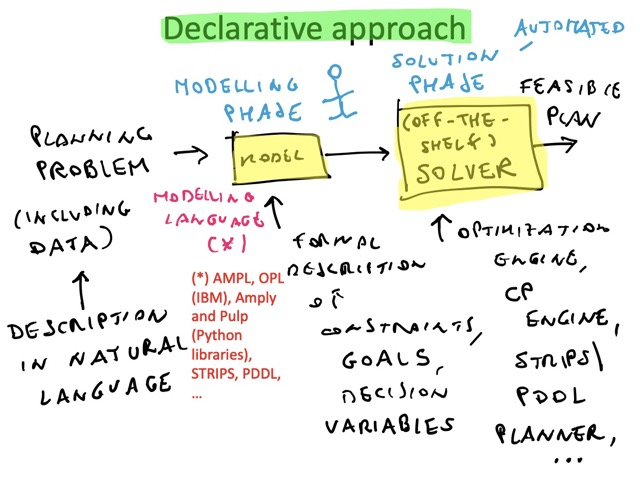
\includegraphics[scale=0.8]{descapp.jpeg}
\caption{procedura implementata} 
\label{descapp}
\end{figure}


Il che è utile dato che \hl{per agire su un problema basterà cambiare il modello} senza cambiare solver, dovrò solo cambiare il modello. È la soluzione più \hl{economico e flessibile} ma è \hl{meno performante} se in ambienti realtime devo prendere soluzioni in tempi molto stretti. Quindi in questi casi servono approcci procedurali.

Per sistemi che devono prendere soluzioni nel breve, si usa \textbf{C, C++, C#}.


% Decisioni non strutturate
\subsection{Decisioni non strutturate o destrutturate}

In questo caso \hl{non possiamo automatizzare}, quindi:

\begin{enumerate}
	\item tiro fuori i \textbf{dati aggregati}
	\item si creano statistiche con \textbf{modelli di ottimizzazione}
\end{enumerate}

Si usano degli \textbf{spreadsheet} che però non riescono a gestire big data e tendono a generare errori.

Il linguaggio più usato è \textbf{Python} ma non è la soluzione più efficiente per tutte quelle applicazioni dove il tempo di calcolo è importante.


% Decisioni semistrutturate
\subsection{Decisioni semistrutturate}

Vogliamo solo \hl{valutare le prestazione di un sistema}. Un esempio sono i sistemi che \hl{presentano un comportamento random} per motivi:

\begin{enumerate}
	\item i \textbf{server hanno un tempo di risposta} che possiamo modellare
	\item le richieste del sistema \textbf{arrivano in maniera stocastica}
\end{enumerate}

Si usano, in questo caso, \hl{metodi simulativi} tramite dei Visual Interactive Modellling System, \hl{per simulare la rete} per la quale passano le informazioni e i server ognuno con diverse proprietà di ciascun linker.


